\chapter{Lampiran Pengujian Eksperimental}
\label{lamp:B}

\section{Kuesioner}
\label{sec:survey}
Kuesioner diawali dengan pertanyaan :
\begin{figure}[H]
	\centering  
	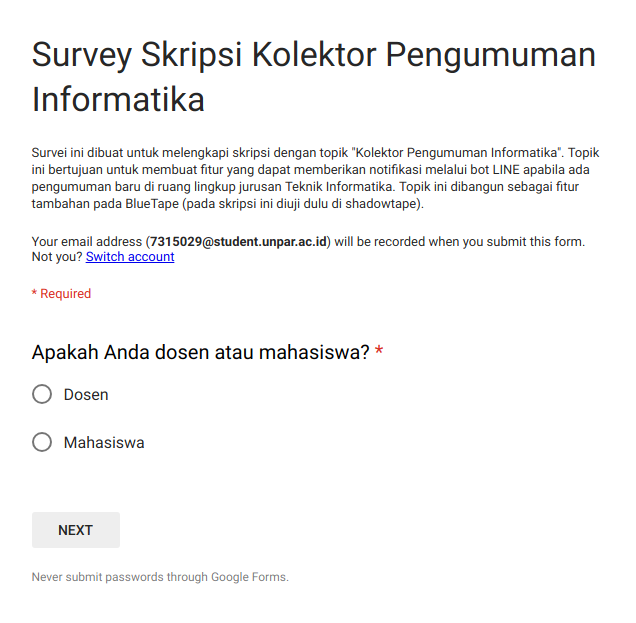
\includegraphics[scale=0.5]{./Survey-Kuesioner/Q0.png}  
	\caption[Kuesioner bagian pertama]{Kuesioner bagian pertama} 
	\label{fig:q0} 
\end{figure}

Apabila responden memilih "Dosen", maka responden akan dialihkan ke bagian Dosen (Lampiran \ref{subsec:survey-dosen}). Apabila responden memilih "Mahasiswa", maka responden akan dialihkan ke bagian Mahasiswa (Lampiran \ref{subsec:survey-mahasiswa}). Responden wajib mengisi semua pertanyaan di kuesioner ini kecuali pertanyaan saran.

\subsection{Dosen}
\label{subsec:survey-dosen}
\begin{figure}[H]
	\centering  
	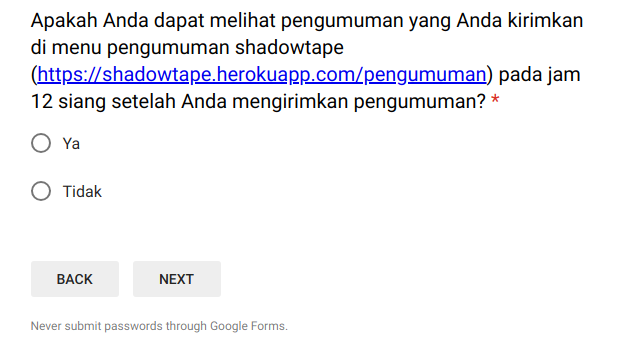
\includegraphics[scale=0.5]{./Survey-Kuesioner/Q1-D1.png}  
	\caption[Kuesioner bagian Dosen pertanyaan pertama]{Kuesioner bagian Dosen pertanyaan pertama} 
	\label{fig:q1-d1} 
\end{figure}

Apabila responden memilih jawaban "Ya" pada pertanyaan pertama (Gambar~\ref{fig:q1-d1}), maka responden akan dialihkan ke pertanyaan kedua (Gambar~\ref{fig:q1-d2}). Apabila responden memilih jawaban "Tidak", maka responden akan dialihkan ke bagian \textit{System Usability Scale} dan Saran (Lampiran \ref{subsec:final}) dan Saran (Gambar~\ref{subsec:final}). 

\begin{figure}[H]
	\centering  
	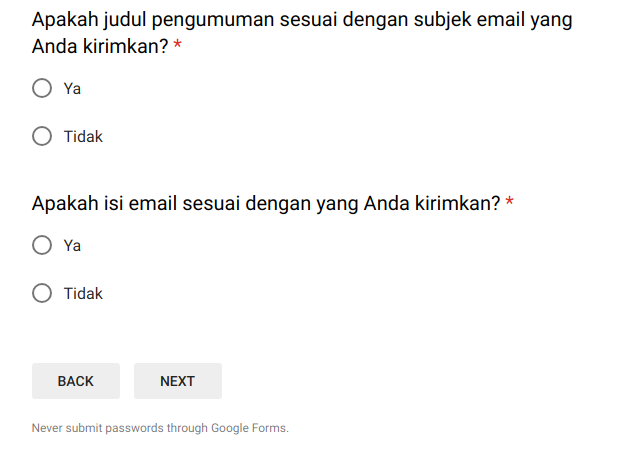
\includegraphics[scale=0.5]{./Survey-Kuesioner/Q1-D2.png}  
	\caption[Kuesioner bagian Dosen pertanyaan kedua dan ketiga]{Kuesioner bagian Dosen pertanyaan kedua dan ketiga} 
	\label{fig:q1-d2} 
\end{figure}

Apabila responden memilih jawaban "Ya" pada pertanyaan ketiga (pertanyaan kedua di Gambar~\ref{fig:q1-d1}), maka responden akan dialihkan ke pertanyaan keempat (Gambar~\ref{fig:q1-d3}). Apabila responden memilih jawaban "Tidak", maka responden akan dialihkan ke bagian \textit{System Usability Scale} dan Saran (Gambar~\ref{subsec:final}). 

\begin{figure}[H]
	\centering  
	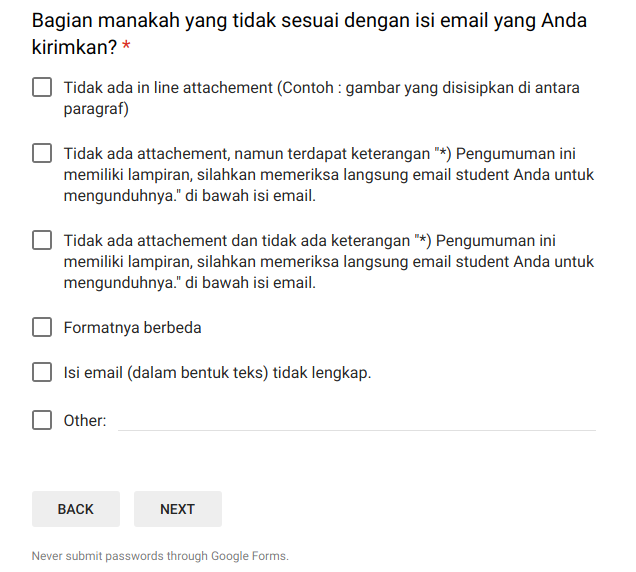
\includegraphics[scale=0.5]{./Survey-Kuesioner/Q1-D3.png}  
	\caption[Kuesioner bagian Dosen pertanyaan keempat]{Kuesioner bagian Dosen pertanyaan keempat} 
	\label{fig:q1-d3} 
\end{figure}

Apapun jawaban responden pada pertanyaan keempat (Gambar~\ref{fig:q1-d3}), responden akan dialihkan ke bagian \textit{System Usability Scale} dan Saran (Gambar~\ref{subsec:final}).

\subsection{Mahasiswa}
\label{subsec:survey-mahasiswa}
\begin{figure}[H]
	\centering  
	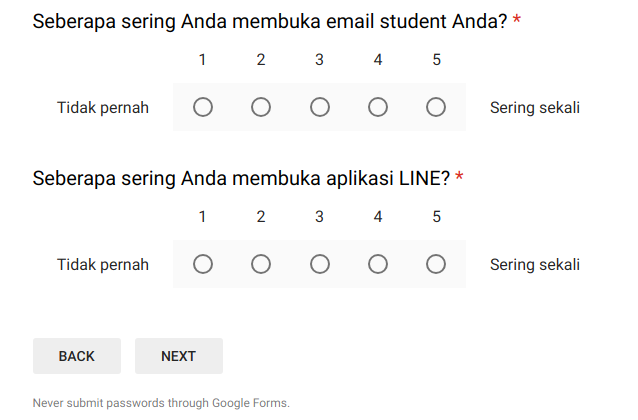
\includegraphics[scale=0.5]{./Survey-Kuesioner/Q1-M1.png}  
	\caption[Kuesioner bagian Mahasiswa pertanyaan pertama dan kedua]{Kuesioner bagian Mahasiswa pertanyaan pertama dan kedua} 
	\label{fig:q1-m1} 
\end{figure}

Apapun jawaban responden pada pertanyaan pertama dan kedua(Gambar~\ref{fig:q1-m1}), responden akan dialihkan ke pertanyaan kedua (Gambar~\ref{fig:q1-m2}).

\begin{figure}[H]
	\centering  
	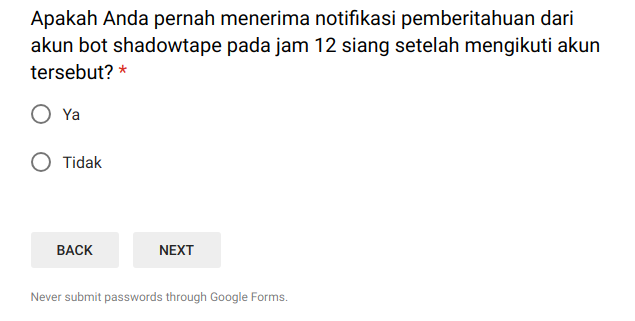
\includegraphics[scale=0.5]{./Survey-Kuesioner/Q1-M2.png}  
	\caption[Kuesioner bagian Mahasiswa pertanyaan ketiga]{Kuesioner bagian Mahasiswa pertanyaan ketiga} 
	\label{fig:q1-m2} 
\end{figure}

Apabila responden memilih jawaban "Ya" pada pertanyaan ketiga (Gambar~\ref{fig:q1-m2}), maka responden akan dialihkan ke pertanyaan keempat (Gambar~\ref{fig:q1-m3}). Apabila responden memilih jawaban "Tidak", maka jawaban responden akan dikirim kepada peneliti.

\begin{figure}[H]
	\centering  
	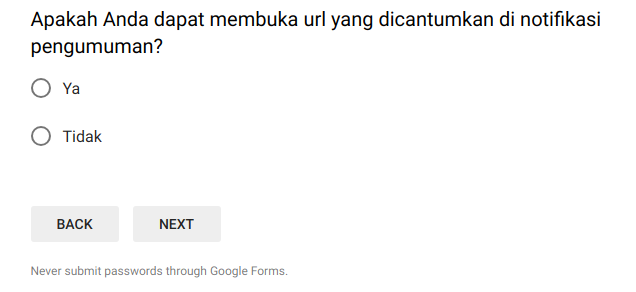
\includegraphics[scale=0.5]{./Survey-Kuesioner/Q1-M3.png}  
	\caption[Kuesioner bagian Mahasiswa pertanyaan keempat]{Kuesioner bagian Mahasiswa pertanyaan keempat} 
	\label{fig:q1-m3} 
\end{figure}

Apabila responden memilih jawaban "Ya" pada pertanyaan keempat (Gambar~\ref{fig:q1-m3}), maka responden akan dialihkan ke pertanyaan kelima (Gambar~\ref{fig:q1-m4}). Apabila responden memilih jawaban "Tidak", maka responden akan dialihkan ke bagian \textit{System Usability Scale} dan Saran (Gambar~\ref{subsec:final}).

\begin{figure}[H]
	\centering  
	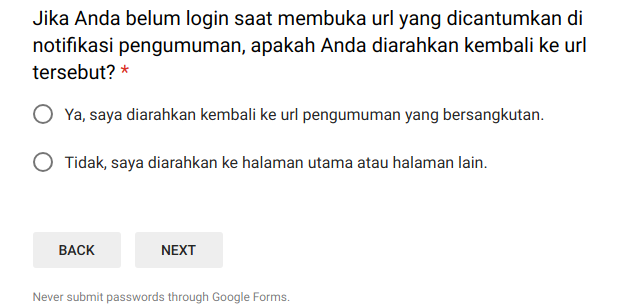
\includegraphics[scale=0.5]{./Survey-Kuesioner/Q1-M4.png}  
	\caption[Kuesioner bagian Mahasiswa pertanyaan kelima]{Kuesioner bagian Mahasiswa pertanyaan kelima} 
	\label{fig:q1-m4} 
\end{figure}

Apapun jawaban responden pada pertanyaan kelima (Gambar~\ref{fig:q1-m4}), responden akan dialihkan ke bagian \textit{System Usability Scale} dan Saran (Gambar~\ref{subsec:final}).

\subsection{\textit{System Usability Scale} dan Saran}
\label{subsec:final}

Bagian ini adalah bagian terakhir dari kuesioner. Bagian ini memiliki 11 pertanyaan yang terdiri dari 10 pertanyaan hasil adaptasi pertanyaan yang ditanyakan saat uji usabilitas dengan metode \textit{System Usability Scale} dan 1 pertanyaan saran. Setelah responden menjawab bagian ini, jawaban responden akan dikirim kepada peneliti. Pertanyaan pada bagian ini ditampilkan pada Gambar~\ref{fig:lq1}, Gambar~\ref{fig:lq2}, dan Gambar~\ref{fig:lq3}.

\begin{figure}[H]
	\centering  
	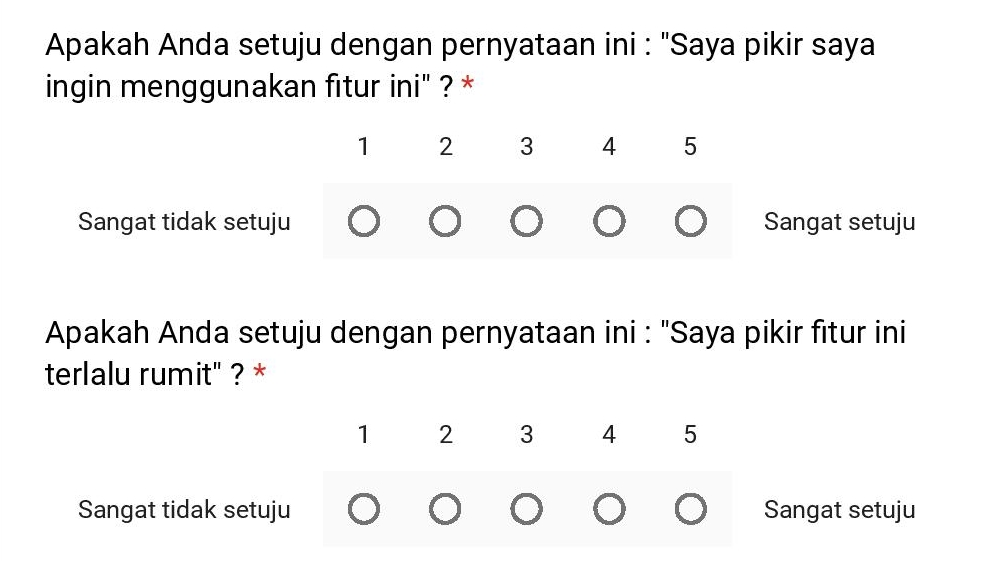
\includegraphics[scale=0.32]{./Survey-Kuesioner/LQ1.jpg} 
	\caption[Kuesioner bagian \textit{System Usability Scale} dan Saran bagian 1]{Kuesioner bagian \textit{System Usability Scale} dan Saran bagian 1} 
	\label{fig:lq1} 
\end{figure}

\begin{figure}[H]
	\centering  
	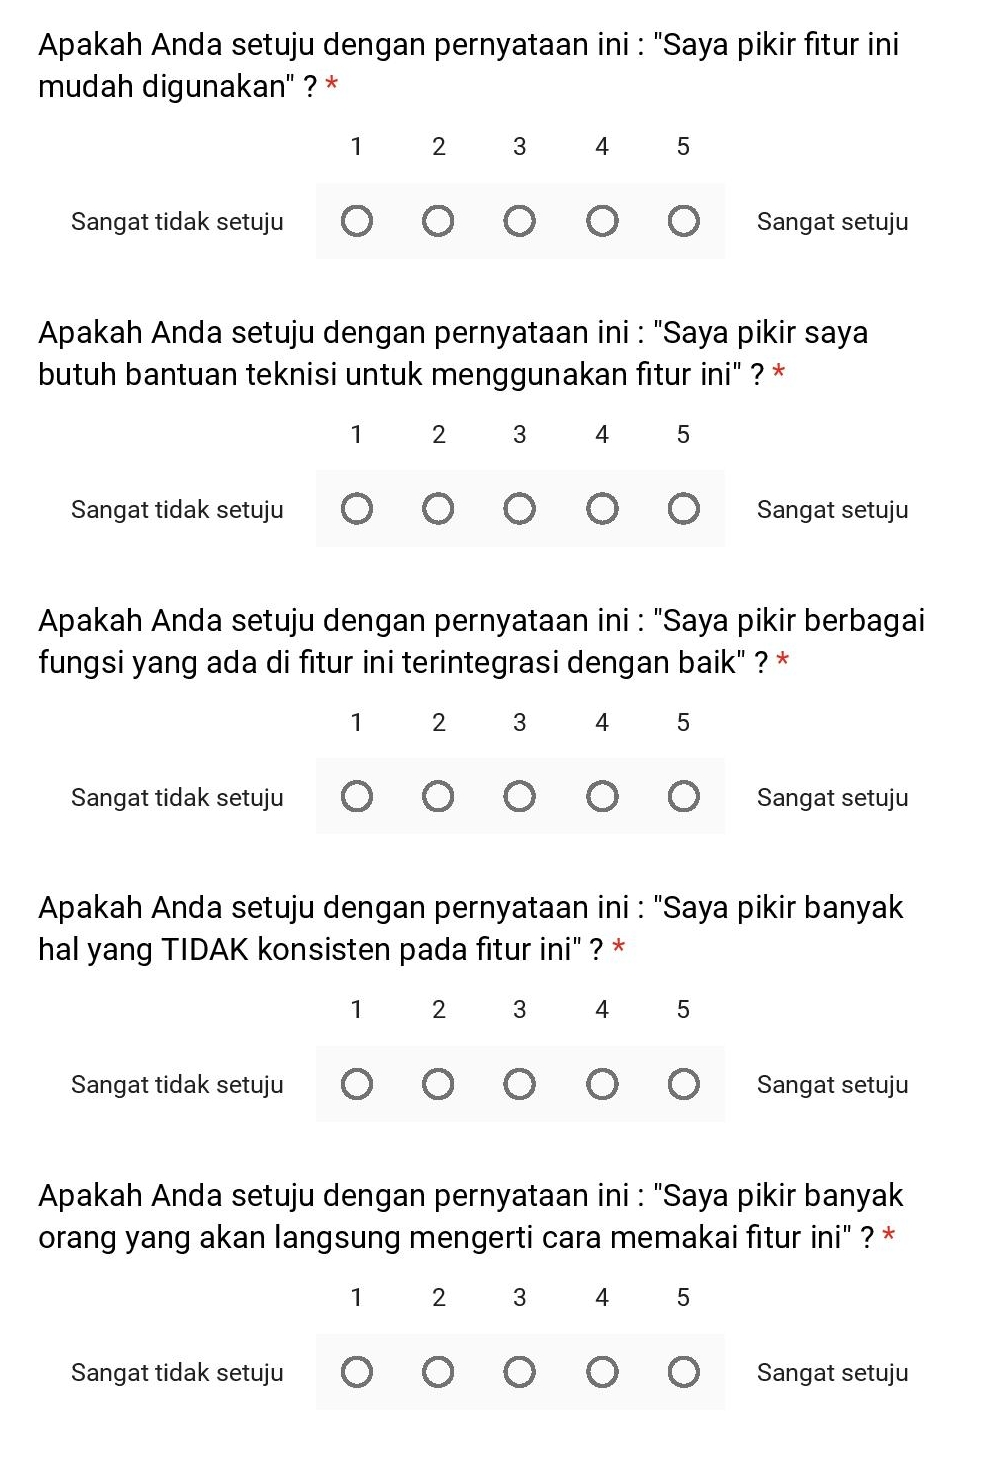
\includegraphics[scale=0.32]{./Survey-Kuesioner/LQ2.jpg}  
	\caption[Kuesioner bagian \textit{System Usability Scale} dan Saran bagian 2]{Kuesioner bagian \textit{System Usability Scale} dan Saran bagian 2} 
	\label{fig:lq2} 
\end{figure}

\begin{figure}[H]
	\centering  
	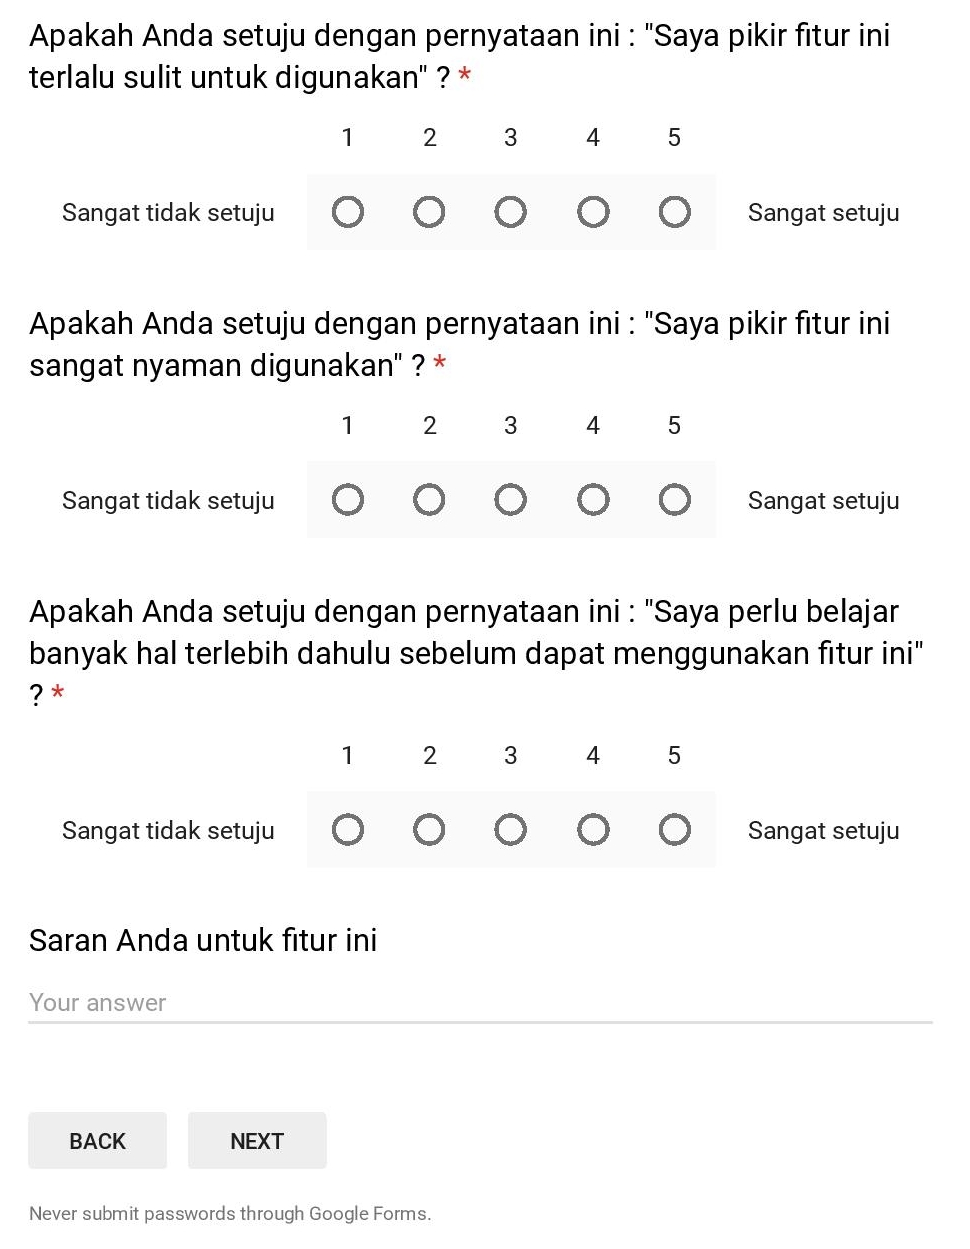
\includegraphics[scale=0.32]{./Survey-Kuesioner/LQ3.jpg}  
	\caption[Kuesioner bagian \textit{System Usability Scale} dan Saran bagian 3]{Kuesioner bagian \textit{System Usability Scale} dan Saran bagian 3} 
	\label{fig:lq3} 
\end{figure}

\label{sec:full-result-survey}
\section{Hasil Mentah Kuesioner}
\begin{table}[H]
	\caption{Hasil Kuesioner Dosen}
	\label{table:hasil-kuesioner-dosen}
	\centering
	\begin{tabular}{|c|c|c|c|c|}
 			\hline
			\textbf{Alamat Email (dianonimkan)} & \textbf{(1)} & \textbf{(2)} & \textbf{(3)}  & \textbf{(4)} \\
			\hline
			b44980@unpar.ac.id & Tidak & - & - & - \\
			\hline
			8759eb@unpar.ac.id & Ya & Ya & Ya & - \\
            \hline
	\end{tabular}
\end{table}
Keterangan:
\begin{itemize}
\item (1): Apakah Anda dapat melihat pengumuman yang Anda kirimkan di menu pengumuman shadowtape (https://shadowtape.herokuapp.com/pengumuman) pada jam 12 siang setelah Anda mengirimkan pengumuman?
\item (2): Apakah judul pengumuman sesuai dengan subjek \textit{email} yang Anda kirimkan?
\item (3): Apakah isi \textit{email} sesuai dengan yang Anda kirimkan?
\item (4): Bagian manakah yang tidak sesuai dengan isi \textit{email} yang Anda kirimkan?
\end{itemize}

\begin{longtable}{|c|c|c|c|c|c|}
	\caption{Hasil Kuesioner Mahasiswa} 
	\label{table:hasil-kuesioner-mahasiswa} \\
\hline
\textbf{Alamat Email (dianonimkan)} & \textbf{(1)} & \textbf{(2)} & \textbf{(3)}  & \textbf{(4)} & \textbf{(5)} \\
\hline	baa288@student.unpar.ac.id	&	3	&	5	&	Ya	&	Tidak	&	-	\\
\hline	30739d@student.unpar.ac.id	&	4	&	5	&	Tidak	&	-	&	-	\\
\hline	da73fa@student.unpar.ac.id	&	4	&	4	&	Tidak	&	-	&	-	\\
\hline	694499@student.unpar.ac.id	&	3	&	5	&	Tidak	&	-	&	-	\\
\hline	c303f0@student.unpar.ac.id	&	3	&	5	&	Tidak	&	-	&	-	\\
\hline	87cdf6@student.unpar.ac.id	&	3	&	5	&	Tidak	&	-	&	-	\\
\hline	890e85@student.unpar.ac.id	&	5	&	5	&	Ya	&	Ya	&	Tidak	\\
\hline	65ba79@student.unpar.ac.id	&	4	&	5	&	Tidak	&	-	&	-	\\
\hline	df46a7@student.unpar.ac.id	&	5	&	5	&	Tidak	&	-	&	-	\\
\hline	5925f0@student.unpar.ac.id	&	2	&	4	&	Tidak	&	-	&	-	\\
\hline	bd86d2@student.unpar.ac.id	&	2	&	4	&	Tidak	&	-	&	-	\\
\hline	7d9892@student.unpar.ac.id	&	4	&	5	&	Ya	&	Tidak	&	-	\\
\hline	f5571c@student.unpar.ac.id	&	5	&	5	&	Tidak	&	-	&	-	\\
\hline	65b189@student.unpar.ac.id	&	5	&	3	&	Tidak	&	-	&	-	\\
\hline	8ba81c@student.unpar.ac.id	&	5	&	5	&	Tidak	&	-	&	-	\\
\hline	70d55b@student.unpar.ac.id	&	5	&	5	&	Ya	&	Ya	&	Ya	\\
\hline	213f43@student.unpar.ac.id	&	5	&	5	&	Ya	&	Tidak	&	-	\\
\hline	77385b@student.unpar.ac.id	&	5	&	5	&	Tidak	&	-	&	-	\\
\hline	489d47@student.unpar.ac.id	&	5	&	5	&	Tidak	&	-	&	-	\\
\hline	52b6e8@student.unpar.ac.id	&	3	&	5	&	Tidak	&	-	&	-	\\
\hline	099027@student.unpar.ac.id	&	5	&	5	&	Ya	&	Ya	&	Tidak	\\
\hline	67ae59@student.unpar.ac.id	&	4	&	5	&	Tidak	&	-	&	-	\\
\hline	f0d182@student.unpar.ac.id	&	3	&	4	&	Ya	&	Ya	&	Ya	\\
\hline	2de1ac@student.unpar.ac.id	&	4	&	5	&	Ya	&	Ya	&	Ya	\\
\hline	c2dd4f@student.unpar.ac.id	&	5	&	5	&	Tidak	&	-	&	-	\\
\hline	0515ae@student.unpar.ac.id	&	2	&	5	&	Ya	&	Ya	&	Tidak	\\
\hline	70047b@student.unpar.ac.id	&	3	&	4	&	Ya	&	Ya	&	Tidak	\\
\hline	126f82@student.unpar.ac.id	&	4	&	5	&	Ya	&	Ya	&	Ya	\\
\hline	80bdb4@student.unpar.ac.id	&	3	&	2	&	Ya	&	Ya	&	Tidak	\\
\hline	2f0c1a@student.unpar.ac.id	&	3	&	5	&	Ya	&	Tidak	&	-	\\
\hline	0f13c2@student.unpar.ac.id	&	4	&	4	&	Ya	&	Ya	&	Ya	\\
\hline	8c6eea@student.unpar.ac.id	&	4	&	4	&	Ya	&	Ya	&	Tidak	\\
\hline	355153@student.unpar.ac.id	&	3	&	4	&	Ya	&	Ya	&	Ya	\\
\hline	22e616@student.unpar.ac.id	&	5	&	5	&	Ya	&	Ya	&	Ya	\\
\hline	0ca428@student.unpar.ac.id	&	3	&	4	&	Tidak	&	-	&	-	\\
\hline	c8d674@student.unpar.ac.id	&	4	&	4	&	Ya	&	Tidak	&	-	\\
\hline	da162a@student.unpar.ac.id	&	3	&	4	&	Tidak	&	-	&	-	\\
\hline	0e388d@student.unpar.ac.id	&	5	&	5	&	Tidak	&	-	&	-	\\
\hline	0ae60f@student.unpar.ac.id	&	2	&	5	&	Tidak	&	-	&	-	\\
\hline	54aa34@student.unpar.ac.id	&	4	&	5	&	Tidak	&	-	&	-	\\
\hline	e63be3@student.unpar.ac.id	&	4	&	5	&	Tidak	&	-	&	-	\\
\hline	f30b7a@student.unpar.ac.id	&	3	&	4	&	Tidak	&	-	&	-	\\
\hline	67e4b0@student.unpar.ac.id	&	4	&	5	&	Ya	&	Tidak	&	-	\\
\hline	7a74ad@student.unpar.ac.id	&	5	&	5	&	Ya	&	Ya	&	Ya	\\
\hline	3dc80d@student.unpar.ac.id	&	3	&	5	&	Tidak	&	-	&	-	\\
\hline	84e410@student.unpar.ac.id	&	4	&	5	&	Ya	&	Ya	&	Ya	\\
\hline	d9bd7e@student.unpar.ac.id	&	5	&	5	&	Ya	&	Ya	&	Tidak	\\
\hline	8b4214@student.unpar.ac.id	&	2	&	5	&	Ya	&	Ya	&	Tidak	\\
\hline	10a358@student.unpar.ac.id	&	3	&	5	&	Tidak	&	-	&	-	\\
\hline	b4dd92@student.unpar.ac.id	&	4	&	5	&	Ya	&	Ya	&	Ya	\\
\hline	2932f4@student.unpar.ac.id	&	5	&	5	&	Ya	&	Tidak	&	-	\\
\hline	9e3e26@student.unpar.ac.id	&	5	&	5	&	Ya	&	Ya	&	Ya	\\
\hline	72d447@student.unpar.ac.id	&	5	&	5	&	Tidak	&	-	&	-	\\
\hline	d1acef@student.unpar.ac.id	&	5	&	5	&	Ya	&	Ya	&	Ya	\\
\hline	9f542d@student.unpar.ac.id	&	4	&	5	&	Ya	&	Tidak	&	-	\\
\hline	35e573@student.unpar.ac.id	&	5	&	5	&	Ya	&	Tidak	&	-	\\
\hline	945aa3@student.unpar.ac.id	&	3	&	5	&	Ya	&	Ya	&	Ya	\\
\hline	8676ec@student.unpar.ac.id	&	5	&	5	&	Ya	&	Ya	&	Ya	\\
\hline	887a27@student.unpar.ac.id	&	4	&	5	&	Ya	&	Tidak	&	-	\\
\hline	66ccab@student.unpar.ac.id	&	5	&	5	&	Ya	&	Tidak	&	-	\\
\hline	ab786d@student.unpar.ac.id	&	3	&	3	&	Ya	&	Ya	&	Ya	\\
\hline	0b62ed@student.unpar.ac.id	&	5	&	5	&	Ya	&	Ya	&	Ya	\\
\hline	fa0a7c@student.unpar.ac.id	&	5	&	5	&	Ya	&	Tidak	&	-	\\
\hline	bfee6e@student.unpar.ac.id	&	3	&	5	&	Ya	&	Ya	&	Tidak	\\
\hline	d79022@student.unpar.ac.id	&	4	&	4	&	Ya	&	Ya	&	Ya	\\
\hline	2fced5@student.unpar.ac.id	&	4	&	5	&	Ya	&	Ya	&	Ya	\\
\hline	ceb5b3@student.unpar.ac.id	&	4	&	5	&	Ya	&	Ya	&	Ya	\\
\hline	b9ce36@student.unpar.ac.id	&	4	&	5	&	Ya	&	Ya	&	Ya	\\
\hline	7c4fc0@student.unpar.ac.id	&	4	&	4	&	Tidak	&	-	&	-	\\
\hline	8d0c41@student.unpar.ac.id	&	4	&	5	&	Ya	&	Ya	&	Ya	\\
            \hline
\end{longtable}
Keterangan:
\begin{itemize}
\item (1): Seberapa sering Anda membuka \textit{email student} Anda?
\item (2): Seberapa sering Anda membuka aplikasi LINE?
\item (3): Apakah Anda pernah menerima notifikasi pemberitahuan dari akun bot shadowtape pada jam 12 siang setelah mengikuti akun tersebut?
\item (4): Apakah Anda dapat membuka \textit{url} yang dicantumkan di notifikasi pengumuman?
\item (5): Jika Anda belum \textit{login} saat membuka \textit{url} yang dicantumkan di notifikasi pengumuman, apakah Anda diarahkan kembali ke \textit{url} tersebut?
\end{itemize}

\begin{longtable}{|c|c|c|c|c|c|c|c|c|c|c|}
	\caption{Hasil Kuesioner System Usability Scale (SUS)} 
	\label{table:hasil-kuesioner-sus} \\
\hline
\textbf{Alamat Email (dianonimkan)} & \textbf{(1)} & \textbf{(2)} & \textbf{(3)}  & \textbf{(4)} & \textbf{(5)} & \textbf{(6)} & \textbf{(7)} & \textbf{(8)} & \textbf{(9)} & \textbf{(10)} \\
\hline	baa288@student.unpar.ac.id	&	4	&	2	&	4	&	4	&	3	&	2	&	4	&	1	&	4	&	2	\\
\hline	b44980@unpar.ac.id	&	5	&	1	&	5	&	1	&	3	&	3	&	5	&	1	&	5	&	1	\\
\hline	890e85@student.unpar.ac.id	&	4	&	3	&	4	&	2	&	4	&	3	&	4	&	2	&	4	&	2	\\
\hline	7d9892@student.unpar.ac.id	&	3	&	3	&	3	&	4	&	3	&	3	&	3	&	3	&	3	&	3	\\
\hline	70d55b@student.unpar.ac.id	&	4	&	2	&	4	&	4	&	4	&	3	&	3	&	2	&	4	&	4	\\
\hline	213f43@student.unpar.ac.id	&	4	&	2	&	4	&	3	&	3	&	3	&	3	&	3	&	3	&	3	\\
\hline	099027@student.unpar.ac.id	&	4	&	4	&	4	&	3	&	4	&	3	&	5	&	2	&	3	&	2	\\
\hline	f0d182@student.unpar.ac.id	&	3	&	2	&	2	&	1	&	4	&	3	&	3	&	3	&	3	&	3	\\
\hline	2de1ac@student.unpar.ac.id	&	4	&	3	&	4	&	4	&	4	&	3	&	4	&	4	&	3	&	4	\\
\hline	0515ae@student.unpar.ac.id	&	3	&	4	&	3	&	1	&	3	&	3	&	4	&	2	&	3	&	3	\\
\hline	70047b@student.unpar.ac.id	&	3	&	4	&	3	&	3	&	2	&	3	&	3	&	3	&	3	&	3	\\
\hline	126f82@student.unpar.ac.id	&	4	&	4	&	4	&	4	&	4	&	4	&	4	&	4	&	4	&	4	\\
\hline	80bdb4@student.unpar.ac.id	&	3	&	3	&	3	&	3	&	3	&	3	&	3	&	3	&	3	&	4	\\
\hline	2f0c1a@student.unpar.ac.id	&	4	&	2	&	4	&	2	&	4	&	3	&	4	&	2	&	4	&	1	\\
\hline	0f13c2@student.unpar.ac.id	&	4	&	2	&	4	&	2	&	4	&	2	&	4	&	2	&	4	&	2	\\
\hline	8c6eea@student.unpar.ac.id	&	3	&	4	&	4	&	4	&	4	&	4	&	4	&	2	&	4	&	4	\\
\hline	355153@student.unpar.ac.id	&	3	&	2	&	4	&	3	&	4	&	3	&	3	&	2	&	3	&	2	\\
\hline	22e616@student.unpar.ac.id	&	4	&	1	&	3	&	3	&	3	&	2	&	4	&	3	&	3	&	3	\\
\hline	c8d674@student.unpar.ac.id	&	3	&	2	&	4	&	3	&	3	&	3	&	2	&	3	&	2	&	3	\\
\hline	67e4b0@student.unpar.ac.id	&	3	&	3	&	4	&	2	&	3	&	3	&	3	&	3	&	3	&	3	\\
\hline	7a74ad@student.unpar.ac.id	&	5	&	5	&	5	&	5	&	5	&	4	&	4	&	4	&	4	&	5	\\
\hline	84e410@student.unpar.ac.id	&	5	&	1	&	5	&	3	&	3	&	3	&	4	&	2	&	4	&	2	\\
\hline	d9bd7e@student.unpar.ac.id	&	5	&	2	&	2	&	5	&	5	&	3	&	3	&	3	&	3	&	3	\\
\hline	8b4214@student.unpar.ac.id	&	4	&	2	&	4	&	2	&	3	&	3	&	3	&	3	&	4	&	3	\\
\hline	b4dd92@student.unpar.ac.id	&	3	&	3	&	3	&	3	&	3	&	3	&	3	&	3	&	3	&	3	\\
\hline	2932f4@student.unpar.ac.id	&	4	&	4	&	3	&	4	&	2	&	3	&	3	&	3	&	3	&	2	\\
\hline	9e3e26@student.unpar.ac.id	&	4	&	2	&	3	&	3	&	3	&	2	&	4	&	2	&	4	&	4	\\
\hline	d1acef@student.unpar.ac.id	&	3	&	3	&	3	&	3	&	3	&	3	&	3	&	3	&	3	&	3	\\
\hline	9f542d@student.unpar.ac.id	&	4	&	2	&	4	&	2	&	3	&	3	&	3	&	3	&	3	&	2	\\
\hline	35e573@student.unpar.ac.id	&	4	&	3	&	3	&	2	&	3	&	3	&	4	&	2	&	3	&	3	\\
\hline	945aa3@student.unpar.ac.id	&	3	&	3	&	3	&	2	&	3	&	4	&	4	&	4	&	4	&	4	\\
\hline	8676ec@student.unpar.ac.id	&	3	&	2	&	4	&	1	&	4	&	2	&	3	&	2	&	3	&	1	\\
\hline	887a27@student.unpar.ac.id	&	5	&	2	&	4	&	4	&	4	&	2	&	4	&	2	&	4	&	2	\\
\hline	66ccab@student.unpar.ac.id	&	3	&	3	&	4	&	2	&	3	&	4	&	2	&	2	&	3	&	2	\\
\hline	ab786d@student.unpar.ac.id	&	5	&	3	&	4	&	1	&	4	&	3	&	4	&	1	&	4	&	1	\\
\hline	0b62ed@student.unpar.ac.id	&	3	&	3	&	3	&	3	&	3	&	3	&	3	&	3	&	3	&	3	\\
\hline	fa0a7c@student.unpar.ac.id	&	5	&	2	&	4	&	4	&	4	&	3	&	4	&	2	&	3	&	4	\\
\hline	bfee6e@student.unpar.ac.id	&	4	&	3	&	3	&	2	&	2	&	2	&	2	&	2	&	3	&	1	\\
\hline	d79022@student.unpar.ac.id	&	4	&	2	&	5	&	2	&	3	&	2	&	2	&	2	&	4	&	3	\\
\hline	2fced5@student.unpar.ac.id	&	3	&	2	&	3	&	2	&	3	&	2	&	3	&	2	&	3	&	1	\\
\hline	ceb5b3@student.unpar.ac.id	&	4	&	3	&	3	&	4	&	3	&	3	&	3	&	3	&	3	&	3	\\
\hline	b9ce36@student.unpar.ac.id	&	3	&	3	&	3	&	2	&	4	&	2	&	3	&	3	&	3	&	4	\\
\hline	8d0c41@student.unpar.ac.id	&	5	&	3	&	4	&	2	&	4	&	3	&	4	&	3	&	5	&	4	\\
\hline	8759eb@unpar.ac.id	&	4	&	3	&	4	&	2	&	3	&	2	&	4	&	2	&	4	&	2	\\
\hline
\end{longtable}
Keterangan:
\begin{itemize}
\item (1) = Apakah Anda setuju dengan pernyataan ini : "Saya pikir saya ingin menggunakan fitur ini" ?
\item (2) = Apakah Anda setuju dengan pernyataan ini : "Saya pikir fitur ini terlalu rumit" ?
\item (3) = Apakah Anda setuju dengan pernyataan ini : "Saya pikir fitur ini mudah digunakan" ?
\item (4) = Apakah Anda setuju dengan pernyataan ini : "Saya pikir saya butuh bantuan teknisi untuk menggunakan fitur ini" ?
\item (5) = Apakah Anda setuju dengan pernyataan ini : "Saya pikir berbagai fungsi yang ada di fitur ini terintegrasi dengan baik" ?
\item (6) = Apakah Anda setuju dengan pernyataan ini : "Saya pikir banyak hal yang TIDAK konsisten pada fitur ini" ?
\item (7) = Apakah Anda setuju dengan pernyataan ini : "Saya pikir banyak orang yang akan langsung mengerti cara memakai fitur ini" ?
\item (8) = Apakah Anda setuju dengan pernyataan ini : "Saya pikir fitur ini terlalu sulit untuk digunakan" ?
\item (9) = Apakah Anda setuju dengan pernyataan ini : "Saya pikir fitur ini sangat nyaman digunakan" ?
\item (10) = Apakah Anda setuju dengan pernyataan ini : "Saya perlu belajar banyak hal terlebih dahulu sebelum dapat menggunakan fitur ini" ?							
\end{itemize}

\begin{longtable}{|c|p{7cm}|}
	\caption{Hasil Kuesioner Saran} 
	\label{table:hasil-kuesioner-saran} \\
\hline
\hline	\textbf{Alamat Email (dianonimkan)}	&	\centerline{\textbf{Saran Anda untuk fitur ini}}	\\
\hline	b44980@unpar.ac.id	&	Tidak bisa "\textit{add friend}" karena akun telah mencapai batas banyak teman.	\\
\hline	70d55b@student.unpar.ac.id	&	Lebih diperbagus tampilannya sehingga menarik \textit{user} untuk menggunakannya	\\
\hline	0f13c2@student.unpar.ac.id	&	\textit{Good Job}!	\\
\hline	2932f4@student.unpar.ac.id	&	terdapat beberapa \textit{error} dalam \textit{login}, dimana \textit{email} saya (@student.unpar) tidak memiliki akses	\\
\hline	d1acef@student.unpar.ac.id	&	memperbaiki \textit{url login} yang dikirimkan di shadowtape	\\
\hline	66ccabd@student.unpar.ac.id	&	saran saya, usahakan tidak menggunakan aplikasi luar lain seperti LINE. dikarenakan tidak semua orang menggunakan line	\\
\hline	0b62ed@student.unpar.ac.id	&	\textit{Link} yang dibuka langsung dari line tidak memiliki hak akses	\\
\hline	fa0a7c@student.unpar.ac.id	&	Fitur ini bagus, memudahkan mahasiswa dalam menerima notifikasi \textit{email}. Namun, waktunya sebaiknya tidak hanya pada jam 12 siang karena waktu tersebut adalah saat orang-orang makan siang yang mungkin saja sedang tidak membuka \textit{gadget}/aplikasi Line pada khususnya.	\\
\hline	d79022@student.unpar.ac.id	&	\textit{Log in} masih tidak dapat dilakukan, terdapat pernyataan bahwa "alamat \textit{email}" tidak memiliki hak akses ke pengumuman. Contohnya \textit{email} yang saya gunakan "2017730044@student.unpar.ac.id tidak memiliki hak akses ke pengumuman"	\\
\hline	2fced5@student.unpar.ac.id	&	"Lebih \textit{user friendly}
"	\\
\hline
\end{longtable}